%!TEX root = ../authorinstr.tex

\section{CACLA}
A well established algorithm in Reinforcement Learning is Continuous Actor Critic Learning Automaton (CACLA)~\cite{van2007reinforcement}. The algorithm deals with continuous state and action spaces. It implements an Actor Critic system in which both the Actor and Critic are operationalized using a Multi-Layer Perceptron. In an Actor-Critic system, the Actor is responsible for selecting the current action given the policy and the Critic is used in the calculation of the Temporal Difference (TD)-error which drives the learning of the Actor. This method allows for a seperation between the representation of the policy and the value function. The TD learning is characterized by equation \eqref{eq:td}. A visualization of the Actor-Critic system is shown in Figure~\ref{fig:actorcriticsystem}. In Reinforcement Learning problems it is important to be aware of the exploration versus exploitation trade-off; meaning that a decision has to be made between exploration which might improve lead to an improvement of the current policy or simply the current best action according to the policy is selected. An exploration technique that is often used in CACLA is Gaussian Exploration, meaning that an action is calculated around the best action that the current policy provides.  

\begin{equation}
\label{eq:td}
V(S_t) \leftarrow V(S_t) + \alpha[r_{t+1} + \gamma V(S_{t+1}) - V(S_t)]
\end{equation}


\begin{figure}[t]
 \centering 
    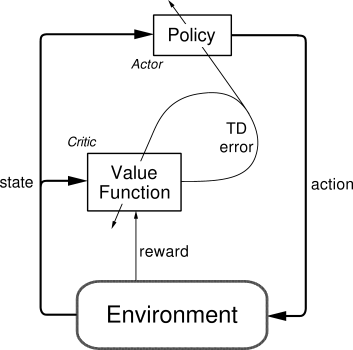
\includegraphics[width = 0.35\columnwidth]{figs/actorcritic.png}
 \caption{Actor Critic system. Reprinted from~\cite{sutton1998reinforcement}}
\label{fig:actorcriticsystem}
\end{figure}



